\documentclass[usenatbib,onecolumn]{mn2e}

\usepackage{amsmath}
\usepackage{graphicx}
\usepackage{epstopdf}

\title{Microlensing as a possible probe of the internal structure of quasars}

\author[Various authors]{[Order TBD] Mihai Tomozeiu$^{1,2}$,Irshad Mohammed,$^1$ Manuel Rabold$^2$,
\newauthor
Prasenjit Saha,$^1$ and Joachim Wambsgans$^3$\\
$^1${Physik-Institut, University of Zurich, Winterthurerstrasse 190,
  8057 Zurich, Switzerland} \\
$^2${Institute for Computational Science, University of Zurich,
  Winterthurerstrasse 190, 8057 Zurich, Switzerland} \\
$^3${Zentrum f\"ur Astronomie der Universi\"at Heidelberg,
  M\"onchhofstrasse 12--14, 69120 Heidelberg, Germany}
}

\begin{document}

\maketitle

\begin{abstract}

In quasars that have been lensed by galaxies, the point-like images
sometimes show sharp brightness variations (microlensing).  These
brightness changes are associated with the innermost region of the
quasar passing behind a complicated pattern of caustics due to the
stars in the lensing galaxy.  In this paper, we study whether the
universal properties of optical caustics could enable extraction of
shape information about the central engine of quasars.  We present a
toy model with a crescent-shaped source crossing a fold caustic.  The
silhouette of a black hole over an accretion disk tends to produce
roughly crescent sources.  When a crescent source crosses a fold
caustic, the resulting light curve is noticeably different from the
case of a disc or Gaussian source.  The crescent parameters, apart
from one degeneracy, can be recovered.
\end{abstract}


\begin{keywords}
Supermassive black holes, microlensing, quasars.
\end{keywords}




%%%%%%%%%%%%%%%%%%%%%%%%%%%%%%%%%%%%%%%%%%%%%%%%%%%%%%%%%%%%%%%%%%%%%%%%%%
\section{introduction}
More than half a century after their discovery, quasars still maintain the interest of a productive part of the astrophysical community. 
Although several mechanisms have been proposed to explain how such systems function, a single mechanism is widely accepted at the present time. 
The model was first proposed by \cite{1964ApJ...140..796S}, followed by \cite{1964SPhD....9..246Z} in the same year and \cite{1969Natur.223..690L} five years later.
The present name of the model is the Super-Massive Black Hole (SMBH) paradigm.\\

According to the paradigm, the object is powered through the accretion of matter from the proximal environment into the black hole. 
The radiation emitted excites the surrounding medium which becomes detectable as the narrow line regions, broad band regions and torus. 
Moreover, in the direction perpendicular to the accretion disk, where the medium is more transparent, jets will appear.
When the medium between and observer and such an object is transparent a quasar can be observed \citep[e.g.,][]{1984RvMP...56..255B}. 
In other words an active galactic nucleus (AGN) with one of the poles orientated towards Earth would be detected as a quasar by an observer. \\

Through extensive observations done in the past 50 years, an important part of the set of assumptions and details  regarding the mechanism have been confirmed and uncovered. 
Still, the black hole shadow and the surrounding luminous accreting material (the black hole silhouette) remain to be probed. 
Advancements in the very long baseline interferometer observations have made possible since 2007, the detection of structures of a few Schwarzschild radii of Sgr~A* at the center of our Galaxy \citep{2008JPhCS.131a2055D}. 
Furthermore, jet launching structure near the supermasve black hole in M87 were resolved with the same observation tool \citep{2012Sci...338..355D}.
With all the advancement, the current number of baselines does not allow the direct generation of images from the observations still it does allow the fitting of the data to predefined models \citep{2013MNRAS.434..765K}.


A whole range of models have been applied starting from simple geometric models to more complex, physically sensible models (\cite{2008Natur.455...78D}, \cite{2011ApJ...738...38B}, \cite{2009ApJ...706..497M}, \cite{2010ApJ...717.1092D}, \cite{2016arXiv160205527F}). 
A significant fraction of the later models predict a crescent shaped silhouette of the black hole. 
This motivated \cite{2013MNRAS.434..765K} to use a simple geometric crescent model to fit the data. 
The succesful results encouraged the authors to speculate that the shadow of the black hole will be observed in the near future with the previously mentioned observation method. \\


Hundreds of thousands of quasars have been detected up to date, mainly from the Sloan Digital Sky Survey. The great majority of them present a redshift larger than 2.15 of their spectra (\citep{2014A&A...563A..54P}). 
Therefore the typical distance to the objects is in the order of gigaparsecs or above. 
A value that is orders of magnitude larger than the distance to M87. The direct observations of the black hole silhouettes of quasars require significant technological advances.\\

We argue in the present paper that one can probe and study the black hole shadow and its proximal environment belonging to a quasar without having to resolve sub-event horizon scales. 
We consider that this is possible by analysing the data from microlensing-events as suggested by \cite{1999ApJ...524...49A}. They argue that if the magnification function $\mu_t(p)$ from equation (6) corresponds to a perfect fold then from the function $F(t)$ present in the same equation one can extract the source profile. We argue in the current article that one can partially 
reconstruct the black hole silhouette up to a simplified crescent geometry. The crescent fit facilitates an estimation of the black hole mass.       
Moreover, unlike with the few nearby AGNs, the study of the very large quasar population allows for the statistical refinement of the global properties of AGN by highlighting any particular
characteristic that is present only in Sgr~A* and M87 central region. 
Furthermore, the probing of the event-horizon-scale inner regions of a large number of objects will facilitate the study of the evolution of the previously mentioned region. \\     
     
Gravitational microlensing of QSOs have been predicted as early as 1981 when \cite{1981ApJ...243..140G} suggested that 
``if haloes of galaxies were composed of stars with masses less than  0.1 $M_\odot$, then these stars acting as individual lenses would produce fluctuations of the order of 
unity in the intensities of the QSO images on time scales of 1 -14 years '' . 
What creates the magnification event is the relative and independent motion of the lens and source with respect to the observer.
Since the respective lens is surrounded by similar objects one would expect to observe during a long enough time interval
multiple microlensing events of the same source, the QSO. 
The sequential alignment of the source and observer with different lensing objects will result in an apparently random increase of the QSO light flux analogous to the scintillation events in a meter of radioactivity.\\

Estimates of the Einstein radius for the particular case of a QSO at redshift 2 lensed by a compact stellar mass object at redshift 0.5 was found to be $10^{-6} \sqrt{M/M_\odot}\rm\,arcsec$ \citep{2001PASA...18..207W}. The Schwarzschild radius of the Sgr A* black hole, situated at 8~kpc from Earth \citep{1993ARA&A..31..345R} spans an angle of 10 microarcsec on the sky \citep{2008JPhCS.131a2055D}. If the quasars observed at $z=2$ would have similar linear sizes, the aparent size of the luminous part of the QSO would be many orders of magnitude below the 1 microarcsec level. Therefore the aparent size would be significantly smaller than the corresponding Einstein radius of a solar mass lens. 
The magnitude differences between the Einstein angle and the aparrent size of the bright part of the QSO motivates the introduction in the first part of the paper of simplified models for     
calculating the lightcurves of QSO magnification events. The simplified models are introduced in the theory section of the present paper. The theory (II) section of the present article starts with an introduction to the basic microlensing theory in which we present the general microlensing equation followed by the concept of magnification. We underline that for the particular case of micro gravitational lensing,
the images are not resolved and thus the magnifications of each images contribute to a total magnification. 
Furthermore, the concept of critical curves and caustics are introduced. Afterwards we focus on a particular catastrophe, namely the fold. 
We choose to study events related to the previously mentioned singularity since the magnification events caused by the crossing of such boundaries are most probable. A quick inspection of figure \ref{fig:magnification_map} by the reader should motivate the previous statement. 
In continuation we introduce the commonly used result involving the magnification of a point-like source near a fold singularity. 
Namely that the magnification is approximately linear outside the caustic and decreases from infinity with the square root of the distance to the boundary when inside the caustic.  
In the last section of the theory (II) we present the general equations for estimating the flux received from an extended source near a fold. 
The only elements required to compute the flux as a function of time are the two dimensional brightness function of the object and the magnification of a point-like source. 
One of the core assumptions made when developing the simple models is that the Einstein angle is orders of magnitude greater than the apparent size of the source. 
Due to this assumption one can imagine the caustic as an infinite wall to be crossed by the source as presented in \ref{fig:infinite_fold}. 
The consequence of the limit is that the information regarding the profiles of the source along any direction parallel to the boundary value is reduced to the corresponding integral value. 
The effect allows the introduction of a one dimensional flux function, which is the two dimensional flux integrated along the axis parallel to the boundary. 
The one dimensional profile contains exhaustively all the information that can be extracted  from the lens generated light-curve \\


In the third section we introduce the three source profiles used in our models and simulations. We start with two commonly used and simple sources. Namely the gaussian brightness distribution and the constant intensity disk. In addition we use a geometric crescent-shaped source effectively the same as the one introduced by \citep{2013MNRAS.434..765K} with constant surface brightness. \\ The fourth section contains the results of our simplified models calculations, including the numerical equation for lightcurve calculations and the corresponding plots. 
In order to facilitate comparison between the lightcurves of the three distinct sources, we constrain the luminosity and half-light radius of all sources to have the same value. 
Furthermore, towards the end of the section, the microlensing light curves were generated for more complex images of black hole silhouettes. 
Namely the images of Sgr A* and M87 compiled in the paper \citep{2015MNRAS.446.1973R} and based on simulations presented in \citep{2009MNRAS.394L.126M} article were used as sources.     
       
We continue to the second part of the paper, where we have advanced the level of complexity of the amplification map. Using the Wambsganss gravitational lensing code \citep{1990LNP...360..186W} a realistic magnification map is generated. The numerical method, hierarchical tree structure and backwards raytracing, underlying the microlensing code is treated in section five. Aside from a basic review of the physical and numerical principles of the code, the description of its generalization from disk shaped source images to crescent ones can be found in the Microlensing code and magnification map as well. Furthermore, the mass distribution in the lens plane, chosen to produce the magnification map used in this analysis, is introduced and motivated.   

In section \ref{sec:fitting}, we carried out a likelihood analysis for the parametrisation of the different source shapes and study the degeneracies involved amongst them. To do so, we mocked the datasets corresponding to each source shape and contaminate them with different noise components. Finally we run MCMC to explore the parameter space of the source shape and some nuisance parameters. The motivation of this part is to explore the possibility if using a simple toy model is it possible to differentiate between symmetric and asymmetric sources based on maximum likelihood analysis. 


Finally, in the Discussion (VII) section, the main results of the current work and their implications are discussed. 



\section{Theory}

\subsection{Basic microlensing theory}

We start by introducing in a succint manner the gravitational lensing theory that is relevant for microlensing in general and for the scope of the
present paper in particular. For a detailed presentation of the theory the reader is referred to the books and articles that represent the references
of the current section (book by Schneider and others). The general microlensing equation can be written as:
\begin{equation}
\vec{y} =   
 \begin{pmatrix}
  1-\gamma - k & 0 \\
  0 & 1 + \gamma -k \\
 \end{pmatrix} 
\vec{x} - \sum_{i=1}^{n} m_i \frac{\vec{x} - \vec{x_i}}{\left( \vec{x} - \vec{x_i} \right)^2}.
\label{eqn:microlensingequation}
\end{equation} 

The equation is valid for a set of $\it{n}$ point (Schwarzschild) lenses placed at coordinates $\vec{x_i}$. $\vec{y}$ represents the coordinates in the source plane for the respective ray, while $\vec{x}$ represents the coordinates in the lens plane. Furthermore, $\gamma$ and $k$ are the shear and surface mass density. For the lens mapping, a Jacobian can be defined:
\begin{equation} 
A(\vec{x}) = 
 \begin{pmatrix}
  \frac{\partial{y_1}}{\partial{x_1}} & \frac{\partial{y_1}}{\partial{x_2}} \\
  \frac{\partial{y_2}}{\partial{x_1}} & \frac{\partial{y_2}}{\partial{x_2}} \\
 \end{pmatrix}. 
\end{equation}
The determinant of $A(\vec{x})$ is related to the local magnification factor through the equation:

\begin{equation}
\mu(\vec{x}) = \left| \frac{1}{det(A(\vec{x}))} \right|
\label{eqn:mu_x}
\end{equation}

According to this equation, from an infinitesimally small source positioned at $\vec{x}$ in the lens plane an observed will receive a flux $\mu(\vec{x}) dF$ instead of the flux $dF$ that would be
observed in the absence of the gravitational lens. In other words the source will dim or brighten depending on whether $\mu(\vec{x})$ is subunitary or supraunitary.\\

In general, for a single infinitesimally small source more than one image can be observed, each with magnification $\mu_j$. For microlensing events the angular sizes of the
images cannot be resolved. The only observable is the flux to which all nearby images contribute. A total magnification
\begin{equation}
 \mu_t = \sum_{j} \mu_j
\end{equation}
 can be defined and account for an increase/decrease of brightness from all images.


\subsection{Magnification of a point source near a fold}

The determinant of the Jacobian $A$ can have both positive and negative values depending in which region it is computed. Such regions are well defined and separated
by critical curves where the determinant vanishes. The lens equation maps the critical curves of the lens plane into caustics in the source plane. An example of the caustic 
shape can be seen in figure \ref{fig:magnification}.\\

\begin{figure}
\centering
  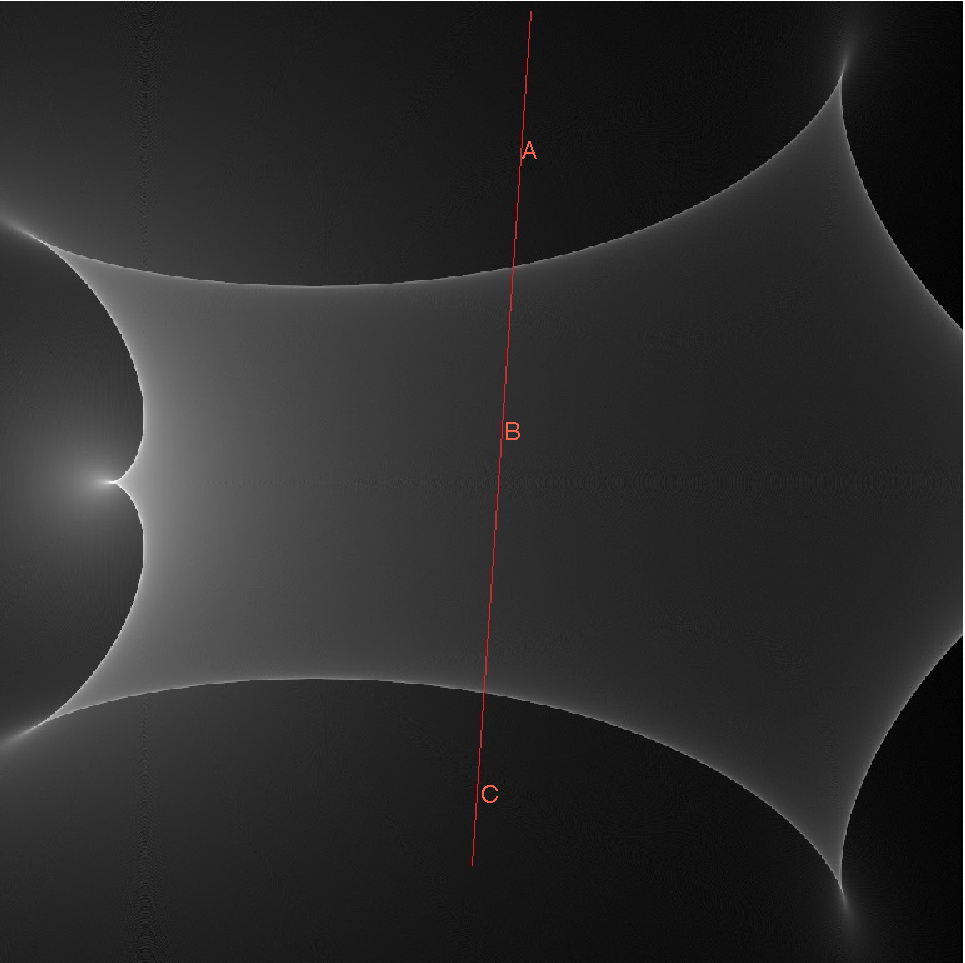
\includegraphics[width=0.95\hsize]{plots/IRIS567_path_2.eps}
\caption{\label{fig:magnification} Magnification map}
\end{figure}

Along these critical curves in the lens plane or caustics in the source plane,  the magnification $\mu$ is infinite, a result that simply follows from equation \ref{eqn:mu_x}. This statement holds only for infinitesimally small sources. For extended sources the maximum amplification is finite since only an infinitesimally small area of the source
overlaps with the caustics \citep{1986BAAS...18T.907S}. 

The matrix $A$ at the coordinates of the caustic can have rank 1 or 0. If the rank is 1 then the coordinates belong to $fold$ or $cusp$ singularities. For the purpose 
of this paper we are interested only in the behaviour around $fold$ singularities. A condition necessary to distinguish between a fold and cusp singularity is that the
eigenvector of $A$ corresponding to the null eigenvalue is not a tangent vector of the critical curve \citep{1992A&A...260....1S}(Dominik 2008).


The behaviour of the images of a point source and their corresponding magnifications near such a caustic has been thoroughly studied in the past. The reader who is interested in 
understanding the details related to this subject is referred to papers such as \cite{1986ApJ...310..568B}, \cite{1992A&A...260....1S}, \cite{2002ApJ...574..970G}, \cite{2002ApJ...580..468G}. For the present paper we only 
summarize the common result:
\begin {equation}
 \mu_{t}(p) = \mu_0 + C_0 \frac{1}{\sqrt{p}} \Theta(p).
\end {equation}
As the previous equation describes the magnification of a point source near a caustic is equal to the sum of the magnification due to other reasons $\mu_0$, assumed to be locally constant,  and a decrease with
the square root of the distance from the fold. The later term becomes activated only after the source enters the region interior to the caustic curves when the values of the stepfunction $\Theta(p)$ become unity. The proportionality
constant $C_0$  is sensible only to the local behaviour of Fermat's potential and units used for the lens plane coordinates $\vec{y}(p,q)$. 

\subsection{Magnification of an extended source near a fold}

A source of arbitrary shape can be described by a two dimensional brightness function $S_{2D}(p - p_s, q - q_s)$ defined for a coordinate system $p,q$ where $p_s, q_s$ denote the coordinates of the center of source.

For a microlensing event the lightcurve can be written for an undefined source shape as:

\begin{equation}
 F(t) = \int_{-\infty}^\infty \int_{-\infty}^\infty S_{2D}(p-p_s(t), q-q_s(t)) \mu_t(p) \mathrm{d}q \mathrm{d}p
 \label{eqn:ft2d}
\end{equation}

In order to build the previous equation we have considered that the time dependency of the flux $F$ is given only by the motion of the source with respect to a fixed caustic. Therefore the only time dependent quantities in the right hand side of the equation
are the coordinates of the center of the source $p_s,q_s$ and by construct $S_{2D}$. 

Due to the choice of the coordinate system the amplification factor has no dependence on the $q$ coordinate. The previous equation can be rewritten as:

\begin{equation}
 F(t) 
= \int_{-\infty}^\infty  \mu_t(p) S_{1D}\left(p-p_s(t)\right) \mathrm{d}p,
\label{eqn:ft}
\end{equation}
\\
where we have defined the one dimensional flux function as:
\begin{equation}
 S_{1D}(p-p_s(t)) = \int_{-\infty}^\infty S_{2D}(p-p_s(t), q-q_s(t)) \mathrm{d}q
\end{equation}

This representation is a valid approximation only when the apparent size of the source is much smaller than the corresponding Einstein angle of the lens. In this context 
all the information about the source shape and brightness that can be contained in the lightcurve is exhaustively given by the 1D flux function.
In other words, if two sources with different $S_{2D}$ have the same $S_{1D}$ they cannot be distinguished by studying their lightcurves.
 
 
\section{Models for extended sources}

In the present study we are analysing three types of sources with different surface brightness: 
\begin{enumerate}
 \renewcommand{\theenumi}{(\arabic{enumi})}
  \item a rotationally symmetric source with a bivariate gaussian surface brightness distribution,
  \item a disk source with constant surface brightness distribution,
  \item a crescent shaped source with constant surface brightness distribution.
\end{enumerate}
The first two sources are the typical choices used in the literature to describe the luminous parts of a quasar (Prasenjit should give some citations here). The third one is a recently proposed
variant \citep{2013MNRAS.434..765K}.




\subsection{Rotationally symmetric source with a bivariate gaussian surface brightness distribution}

A symmetric 2D gaussian can be described mathematically as:

\begin{equation}
 S_{2D}^G(p-p_s, q-q_s) = \frac{S_0^G}{2 \pi \sigma^2} e^{-\frac{(p-p_s)^2}{2 \sigma^2}} e^{-\frac{(q-q_s)^2}{2 \sigma^2}}.
\end{equation}
\\
The corresponding 1D brightness is:

\begin{equation}
 S_{1D}^G(p-p_s) = \frac{S_0^G}{\sqrt{2 \pi} \sigma} e^{-\frac{(p-p_s)^2}{2 \sigma^2}}.
\end{equation}
\\
Other parameters of the model are the total flux $S_0^G$ and $\sigma$. 

Although such a definition for a source would have non-zero surface/linear brightness for any coordinate $p,q$, the amount of light received by a detector from outside a $3 \sigma$ disk centered at $p_s, q_s$ 
would be insignificant. For a gaussian distributed surface brightness source the half-light radius is directly proportional to the parameter $\sigma$ according to the equation:
\begin{equation}
r_{1/2} = \sqrt{ln(4)} \sigma.
\end{equation}

\subsection{Disk source with constant surface brightness distribution}

One can construct mathematically a disk source with constant surface brightness and radius $R$ using a stepfunction:
\begin{equation}
 S_{2D}^D(p-p_s, q-q_s) = \frac{S_0^D}{\pi R^2} \Theta \left( R^2 - \left( p-p_s \right)^2 - \left( q-q_s \right)^2 \right).
\end{equation}
By integrating over $q$ coordinate the linear brightness function is obtained:


\begin{equation}
 S_{1D}^D(p-p_s) = \frac{2 S_0^D}{\pi R}  \sqrt{1 - \frac{(p-p_s)^2}{R^2} }    \Theta \left( R^2 - \left( p-p_s \right)^2 \right).
\end{equation}
\\
The half-light radius of a uniform disk source is $R/\sqrt{2}$.

\subsection{Crescent source with constant surface brightness distribution}

The surface brightness distribution of a geometric crescent can be built by considering two disk sources of constant brightness. One larger disk will contribute positively to the total flux, while one smaller disk 
that is interior to the large one will contribute negatively. This superposition can be written for 2D as:\\

\begin{equation}
 S_{2D}^C =  S_{2D}^{Dp} -  S_{2D}^{Dn}   (n+1)
 \label{eqn:s2d}
\end{equation}
with\\

\begin{equation}
 S_{2D}^{Dp}(p-p_{sn}, q-q_{sn}) = \frac{S_0^{Dp}}{\pi R_p^2} \Theta \left( R_p^2 - \left( p-p_{sp} \right)^2 - \left( q-q_{sp} \right)^2 \right)
\end{equation}
\\
and
\begin{equation}
 S_{2D}^{Dn}(p-p_{sn}, q-q_{sn}) = \frac{S_0^{Dn}}{\pi R_n^2} \Theta \left( R_n^2 - \left( p-p_{sn} \right)^2 - \left( q-q_{sn} \right)^2 \right).
\end{equation}
\\
The following notations were used: $R_p, (p_{sp}, q_{sp}), R_n, (p_{sn},q_{sn})$ are the radii and coordinate of the center for the larger positive disk and smaller negative disk respectively.  $S_0^{Dp},S_0^{Dn}$ represent the total flux of radiation received from the large and small disk. From this point forward we will not use the total flux from each source. Instead we will 
use the difference which in this case is th total flux from the crescent-shaped source $S_0^C$. \\
Equation \ref{eqn:s2d} can be written as:\\

\begin{align}
 S_{2D}^C &= \frac{S_0^C}{\pi \left(R_p^2-R_n^2 \right)} \left\{ \Theta \left[ R_p^2 - \left( p-p_{sp} \right)^2 - \left( q-q_{sp} \right)^2 \right] \right.\nonumber\\
 &\qquad \left. {} -  \Theta \left[ R_n^2 - \left( p-p_{sn} \right)^2 - \left( q-q_{sn} \right)^2 \right] \right\}.
\end{align}
\\
Analogous for the linear brightness function:

\begin{align}
 S_{1D}^C &= \frac{2 S_0^C}{\pi \left(R_p^2-R_n^2 \right)} \left\{ \sqrt{R_p^2 - (p-p_{sp})^2}  \Theta \left[ R_p^2 - \left( p-p_{sp} \right)^2 \right] \right.\nonumber\\
 &\qquad \left. {} - \sqrt{R_n^2 - (p-p_{sn})^2 } \Theta \left[ R_n^2 - \left( p-p_{sn} \right)^2 \right] \right\}.
\end{align}


There are some constraints on the parameters used to define a crescent in the previously presented manner that need to be stated. First, we must impose the obvious $R_p > R_n$ relation. Secondly, 
the small disk must always be interior to the large disk:
\begin{equation}
 R_p \ge R_n + \sqrt{\left(p_{sp} - p_{sn} \right)^2 + \left(q_{sp} - q_{sn} \right)^2}
\end{equation}

For the distances between the centers of the two disks we will use the same notations as the one found in the paper \citep{2013MNRAS.434..765K}, $a \equiv p_{sn} - p_{sp}$ and $b \equiv q_{sn} - q_{sp}$.

The half-light radius of any source is invariant to any rotational transformation. In the present case of a crescent source the effective radius is dependent on the parameters $R_p$, $R_n$ and $\sqrt{a^2+b^2}$ exclusively. From symmetry considerations the centroid of the source is colinear with the centers of the two disks and it is situated at a distance $d_c$ from the center of the brigth disk. $d_c$ can be computed numerically by solving the equation:

\begin{equation}
\frac{S_0^C}{2} =  
\end{equation}   


\begin{figure}
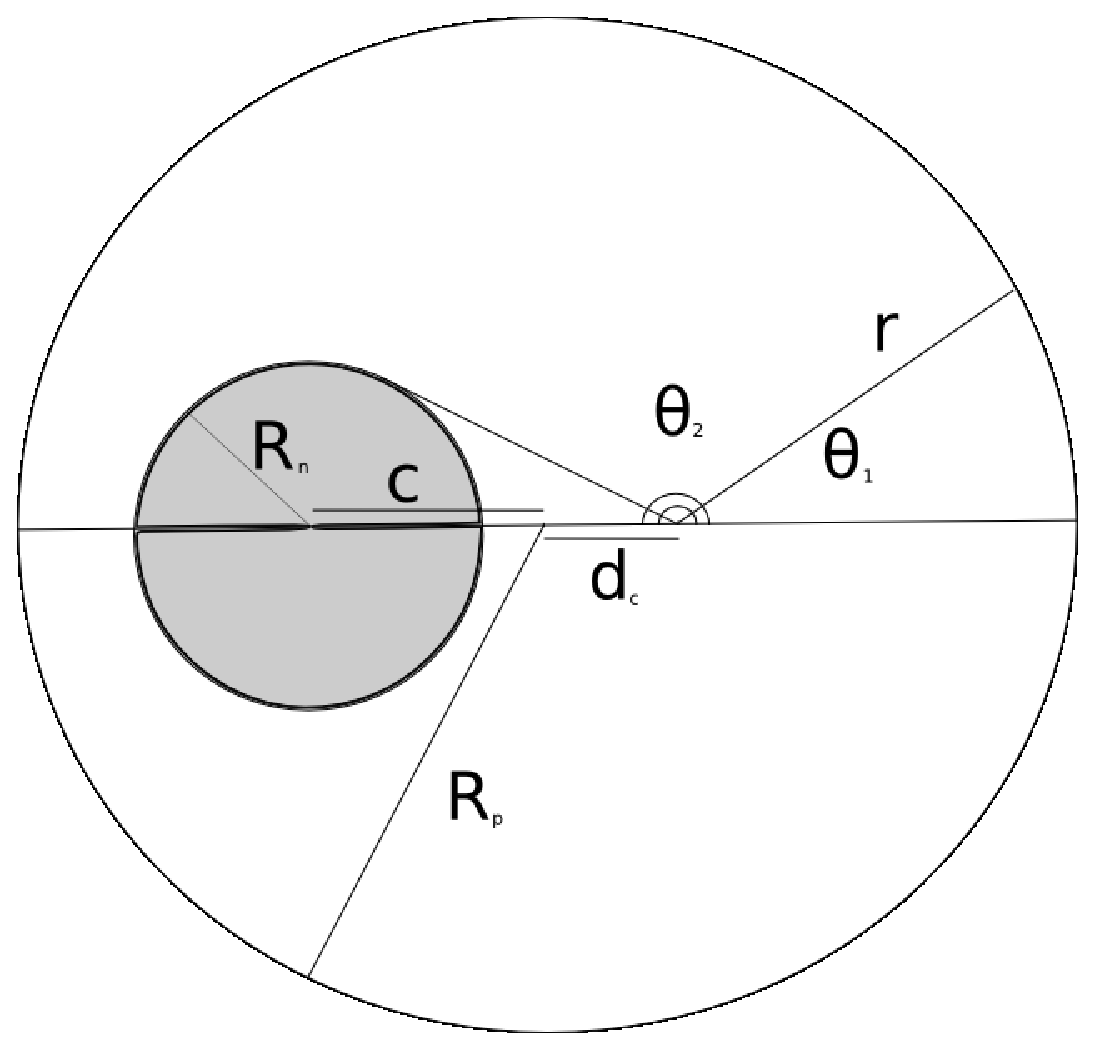
\includegraphics[width = .8\textwidth]{plots/figure_rhalf.eps}
\caption{\label{fig:lightcurve_crescent} Lightcurve ?.}
\end{figure}





\section{Lightcurves of the extended sources during fold crossing}

Using equation \ref{eqn:ft} and the one-dimensional flux function presented in the previous section one can compute numerically the lightcurves of the three extented sources for the simplified 
infinite-wall-caustics model.

\subsection{Lightcurve of the gaussian source}

The amount of light received by an observer from a source with a gaussian distributed brightness with $\sigma$ and total flux $S_0^G$ in the absence of any gravitational lensing is:
\begin{equation}
 F^G(t) = \int_{-\infty}^\infty  \left( \mu_0 + \frac{C_0}{\sqrt{p}} \Theta \left( p \right) \right) \left( \frac{S_0^G}{\sqrt{2 \pi} \sigma} e^{-\frac{(p-p_s(t))^2}{2 \sigma^2}} \right) \mathrm{d}p.
\end{equation}
which can be simplified to:
\begin{equation}
 F^G(t) = \mu_0 S_0^G + \frac{C_0 S_0^G}{\sqrt{2\pi} \sigma} \int_{0}^\infty \frac{e^{-\frac{(p-p_s(t))^2}{2 \sigma^2}}}{\sqrt{p}} \mathrm{d}p.
\end{equation}


\begin{figure}
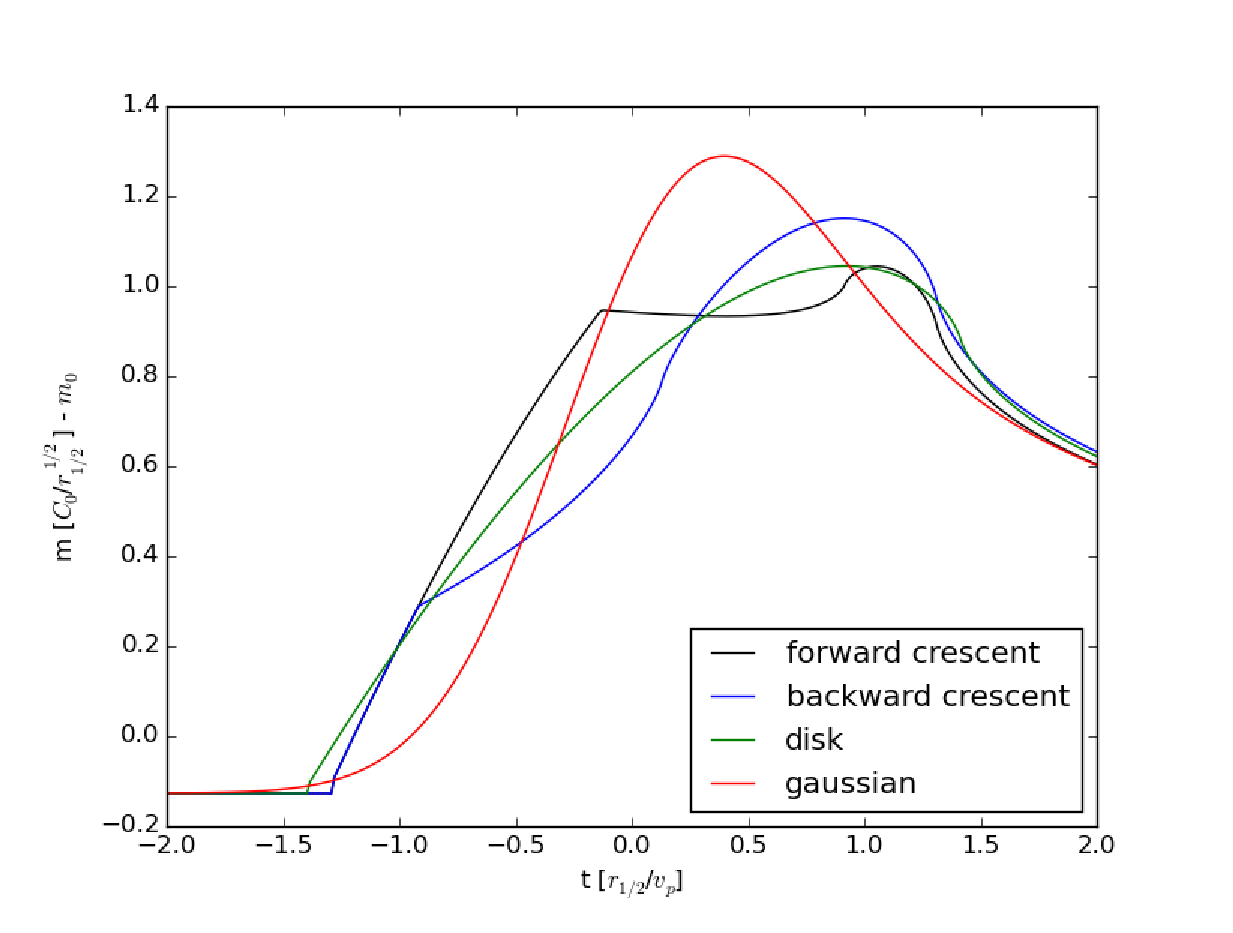
\includegraphics[width = .8\textwidth]{plots/4source_magnification.eps}
\caption{\label{fig:lightcurve_gauss} Lightcurves of crescents, gaussian and disk for sources with identical $S_0$ and $r_{1/2}$. }
\end{figure}


\subsection{Lightcurve of the disk shaped source}

Analogous to the gaussian shaped source, the disk source with uniform brightness, radius $R$ and unmagnified flux $S_0^D$ has a lightcurve described by the equation:

\begin{equation}
 F^D(t) = \int_{-\infty}^\infty  \left( \mu_0 + \frac{C_0}{\sqrt{p}} \Theta \left( p \right) \right) \left( \frac{2 S_0^D}{ \pi R} \sqrt{1 - \frac{\left( p-p_s(t) \right)^2}{R^2}} \Theta \left(R^2 - \left(p-p_s(t) \right)^2 \right) \right) \mathrm{d}p.
\end{equation}

which is equivalent to:
\begin{equation}
 F^D(t) = \mu_0 S_0^D + \frac{2 C_0 S_0^D}{\pi R} \int_{max(0, p_s(t) - R)}^{max(0, p_s(t) + R)} \frac{1}{\sqrt{p}} \sqrt{1 - \frac{\left( p-p_s(t) \right)^2}{R^2}} \mathrm{d}p.
\end{equation}

\begin{figure}
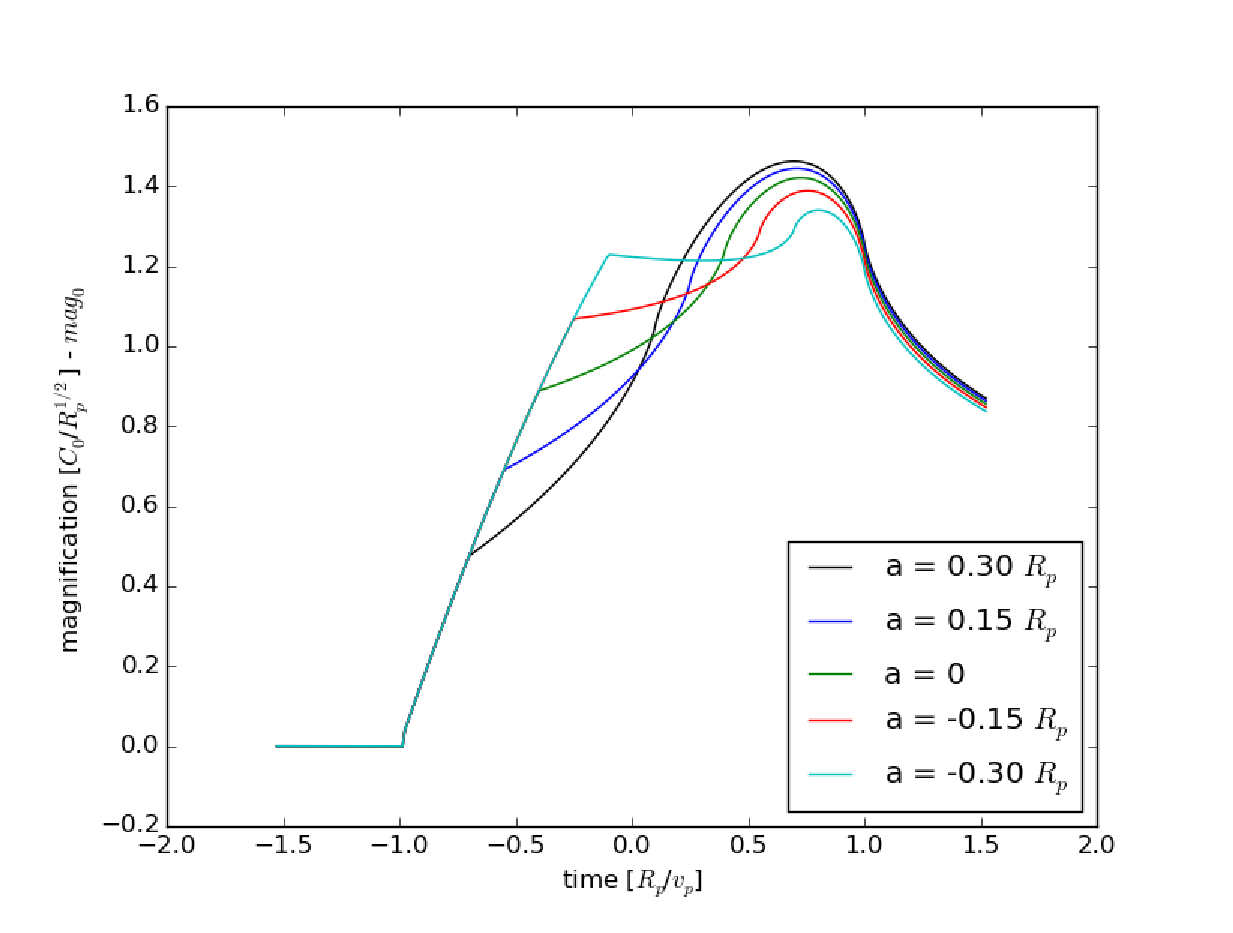
\includegraphics[width = .8\textwidth]{plots/4avar_magnification.eps}
\caption{\label{fig:lightcurve_disk} Lightcurves of crescent with.}
\end{figure}


\subsection{Lightcurve of the crescent shaped source}

The lightcurve of a crescent shaped source with unamplified flux $S_0^C$, radii $R_p$, $R_n$ and center displacement $a(t)$ is:
\begin{equation}
 F^c(t) = \mu_0 S_0^C + C_0 \frac{2 S_0^C}{\pi \left( R_p^2 -R_n^2 \right) } 
\left(\int_{max(0, p_s(t) - R)}^{max(0, p_s(t) + R)} \sqrt{\frac{R_p^2 - \left( p-p_s(t) \right)^2 }{p}} \mathrm{d}p 
  -  \int_{max(0, p_s(t) - a(t) - R)}^{max(0, p_s(t) -a(t) + R)} \sqrt{\frac{R_p^2 - \left( p-p_s(t) +a(t) \right)^2 }{p}}  \mathrm{d}p \right)
\end{equation}


\begin{figure}
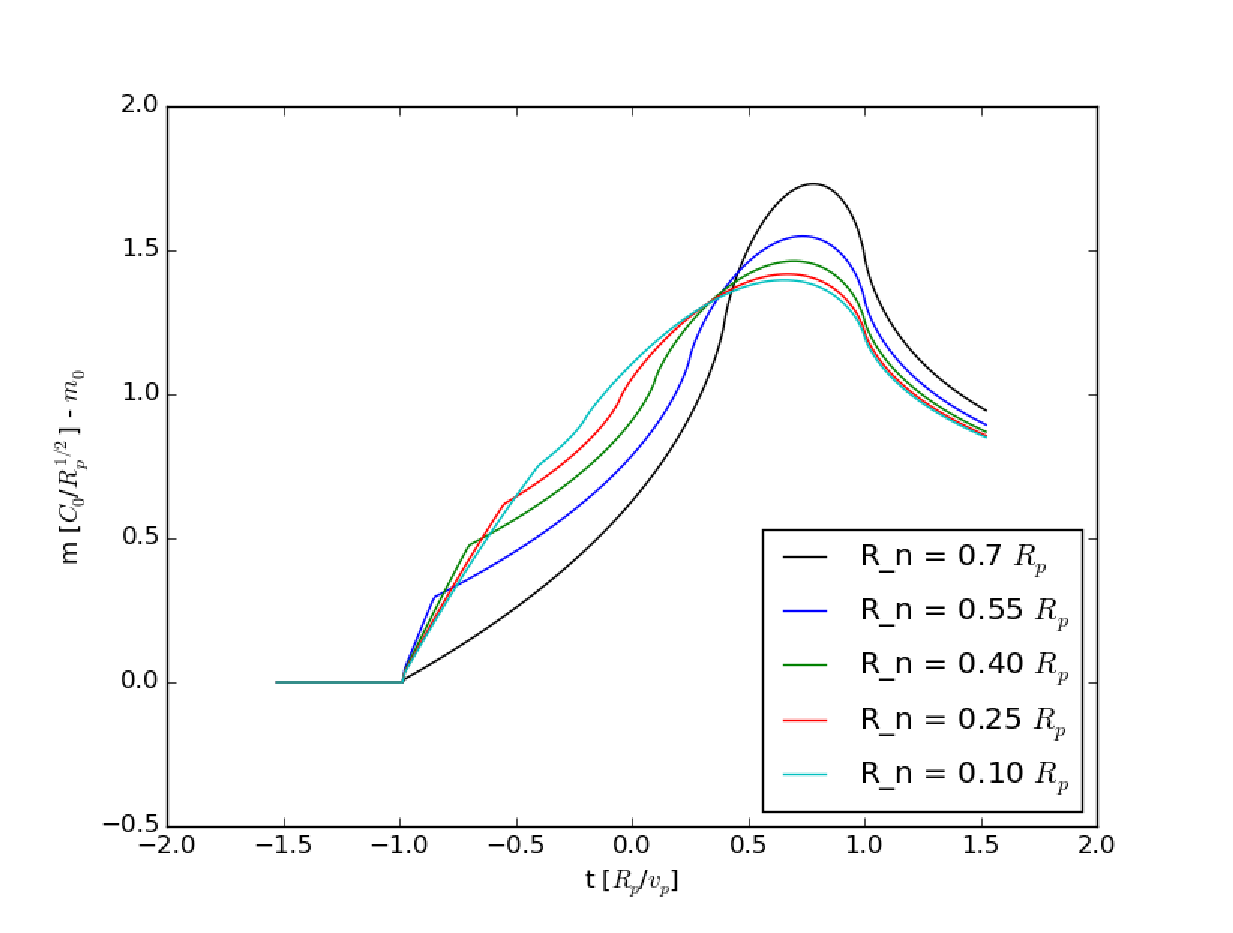
\includegraphics[width = .8\textwidth]{plots/4rn_magnification.eps}
\caption{\label{fig:lightcurve_crescent} Lightcurve 3.}
\end{figure}

The function $p_s(t)$ can be chosen to be equal to $v_p(t-t_0) + p_{s0}$. Where $p_{s0}$ is the coordinate $p$ of the source at the initial time, and $v_p$ is the component of the velocity
along the $p$ axis. Such a modeling of the motion of the object in the source plane describes a linear motion with constant velocity. Furthermore, we reduce the complexity of the model by 
chosing the function $a(t)$ to be constant in time.  

\begin{figure}
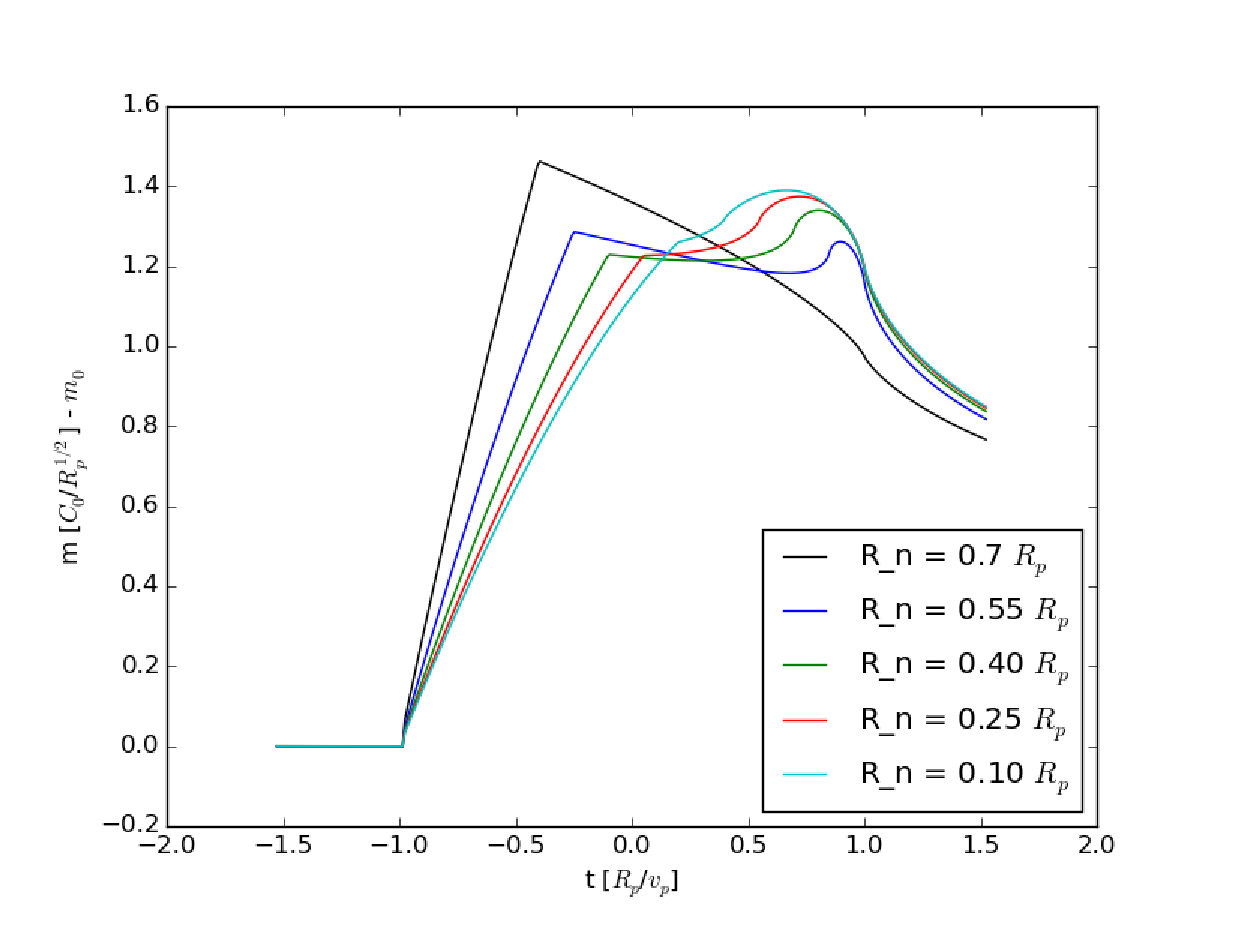
\includegraphics[width = .8\textwidth]{plots/4rn2_magnification.eps}
\caption{\label{fig:lightcurve_crescent} Lightcurve 4.}
\end{figure}



\section{Microlensing code and magnification maps}

\section{Model fitting and likelihood analysis}\label{sec:fitting}

In this section we simulate the fitting of source models to
lightcurves in the presence of random and systematic errors.  We
generate mock data for three source models --- a crescent, a uniform
disc and a Gaussian disc --- and then fit each mock light curve to all
three source models. Parameter fitting and marginalising was done by
Markov-chain Monte Carlo (MCMC).

\begin{figure}
\centering
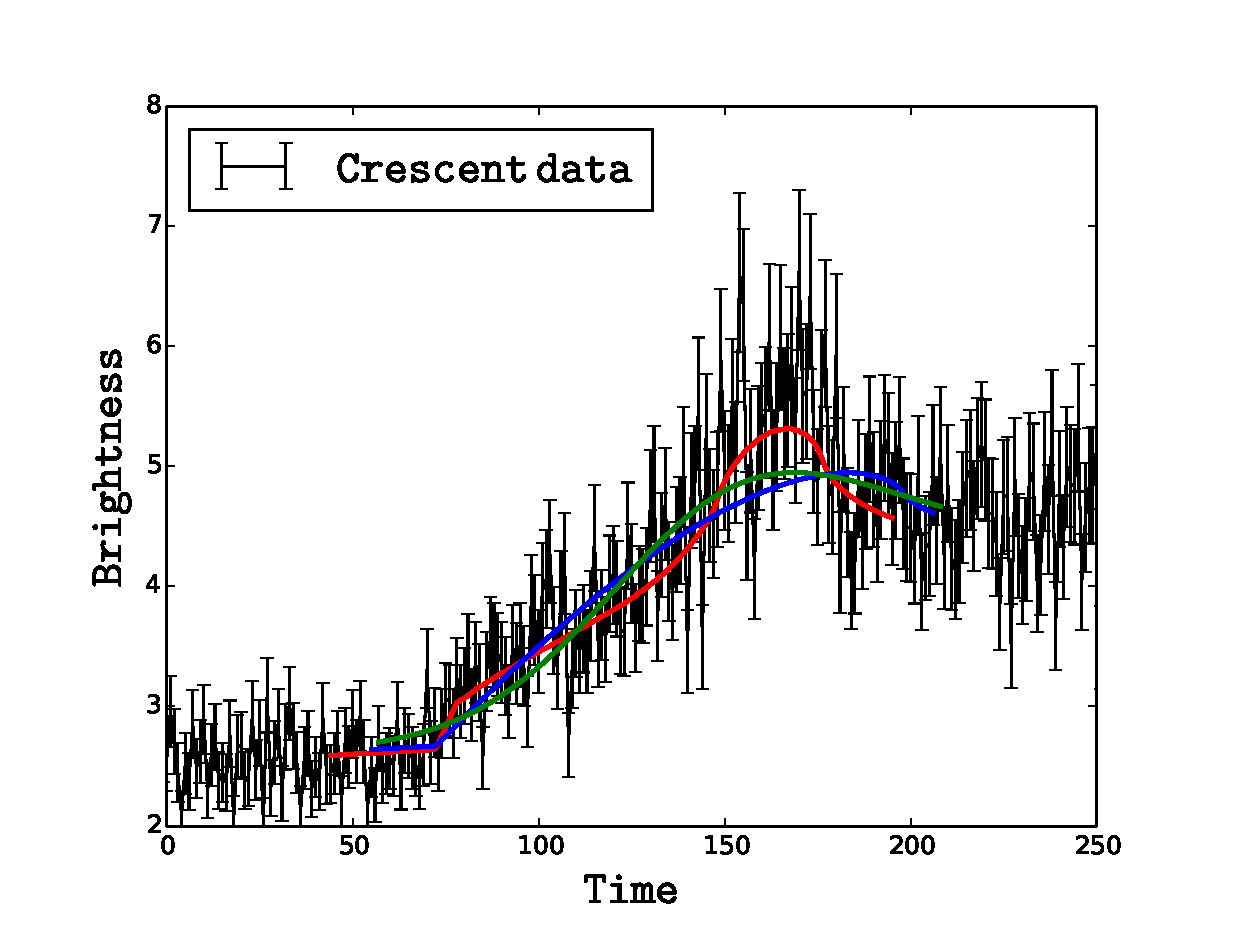
\includegraphics[width=0.9\hsize,bb=0 0 576 432
                ]{plots/data_cc.eps}
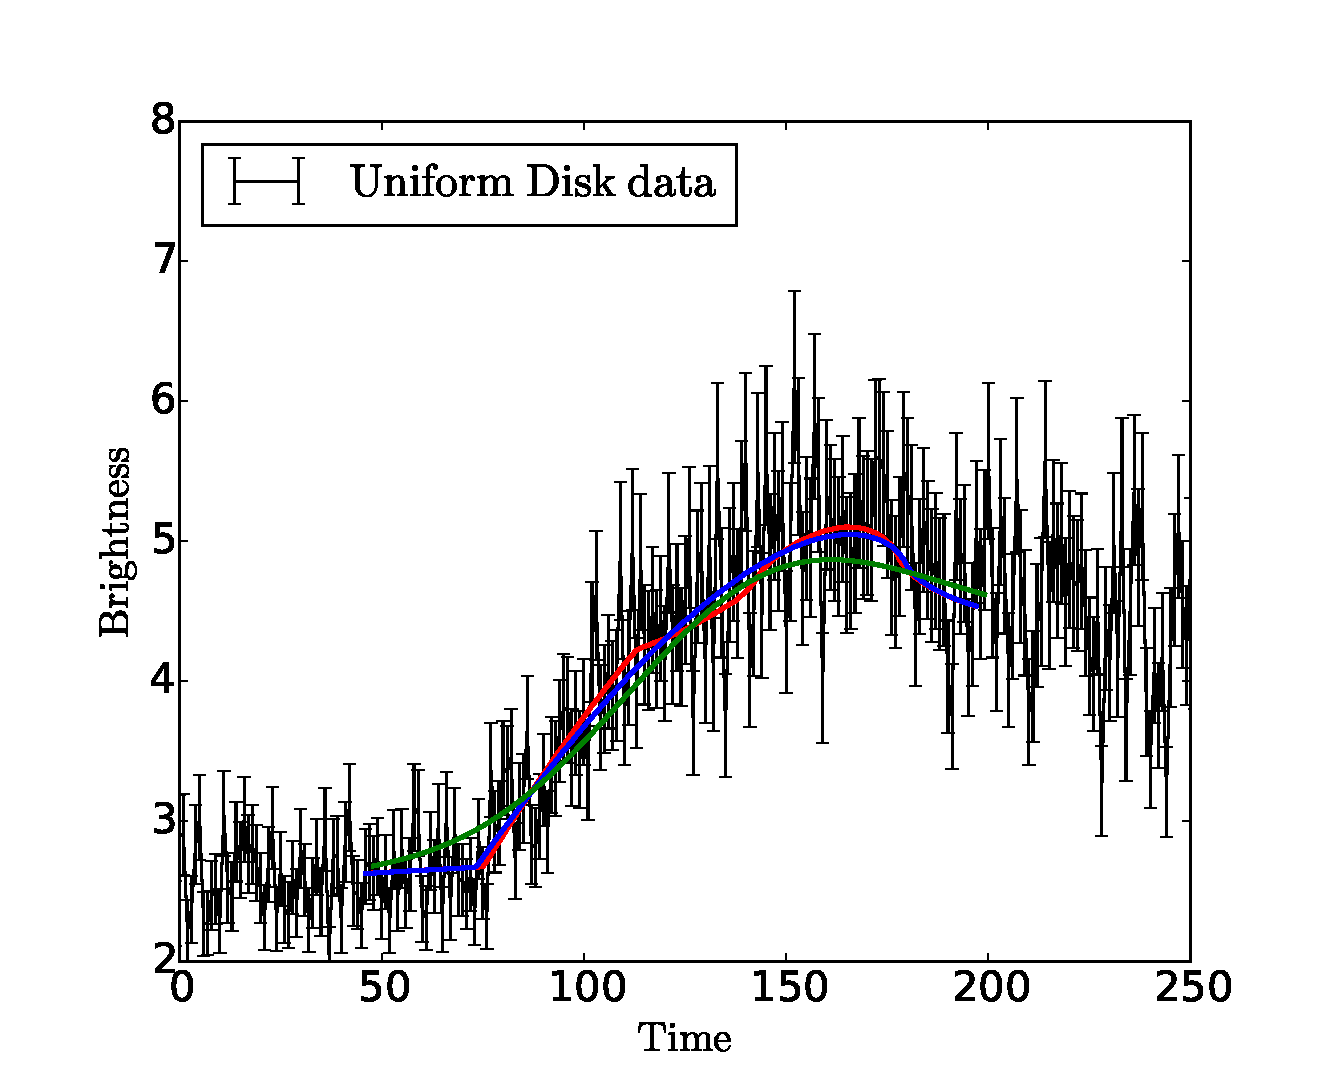
\includegraphics[width=0.9\hsize,bb=0 0 576 432
                ]{plots/data_dd.eps}
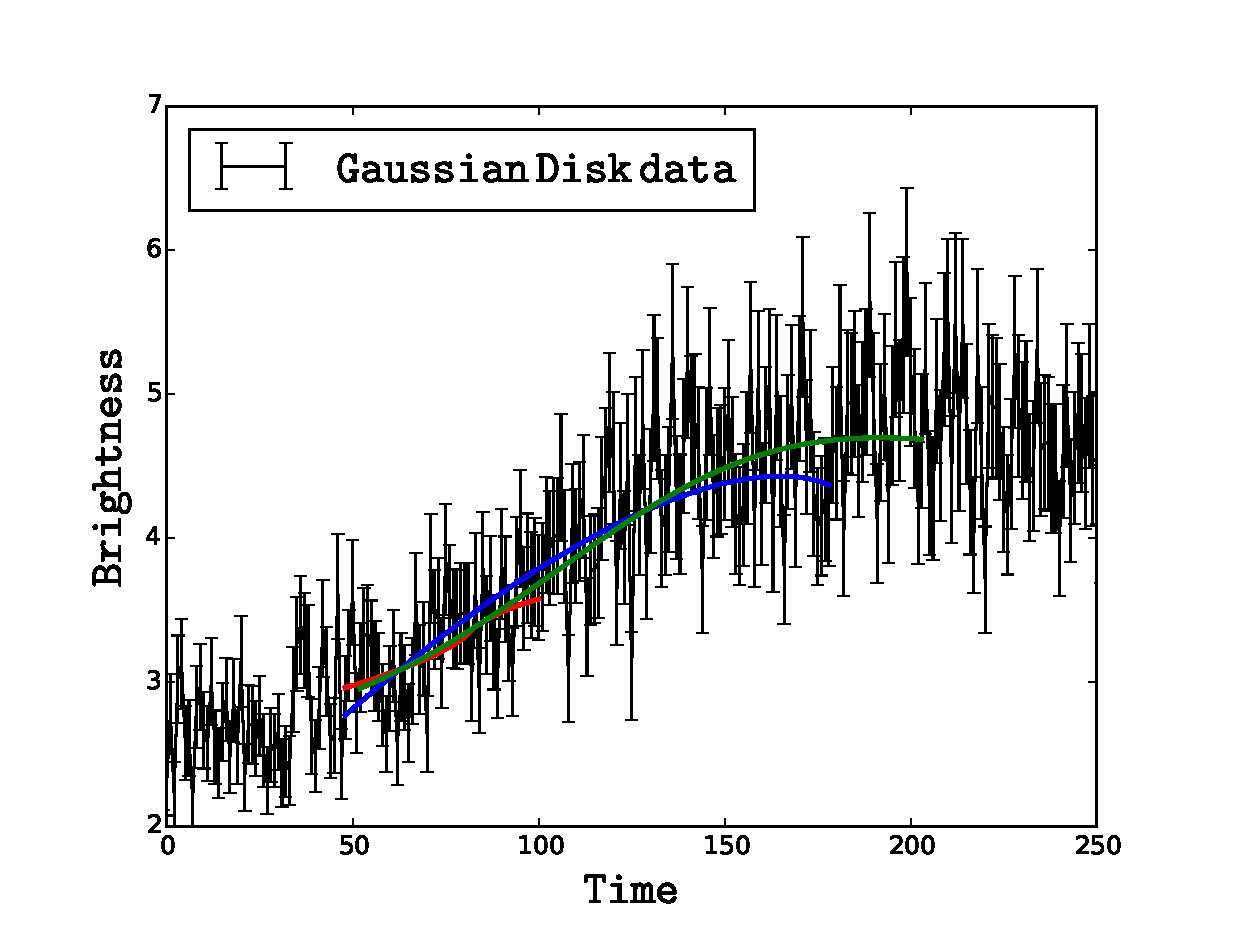
\includegraphics[width=0.9\hsize,bb=0 0 576 432
                ]{plots/data_gg.eps}
\caption{\label{fig:mockdata} Three different mock datasets with
  three different parametrizations fitted to each --- crescent (red),
  uniform-disk (blue) and Gaussian disk (green).}
\end{figure}

\subsection{Mock datasets}

Mock light curves were generated by running a source across a
caustic, specifically along the line from point C to point B in
Figure~\ref{fig:magnification_map}.  The model light curves, to which
these are fitted, are made by running a source across a different
caustic, along the line from point A to point B in the same figure.
That is, the mock data are generated with a clean but not ideal fold
caustic and then fitted with another such caustic.  This mimics the
unavoidable systematic error of not knowing the caustic exactly.

The crescent source had parameters (as explained in
\S\ref{subsec:crescent}) $R_p$ and $R_n$ being the radii of the outer
and inner circles and $(\alpha,\beta)$ being the coordinates of the inner
circle with respect to the centre of the outer circle in the coordinate system associated with the image in Figure 1 and not associated 
with the caustic surface as defined in the previous sections.  The parameter values were
\begin{equation}
   (R_p, R_n, \alpha, \beta) = (50.0, 30.0, 15.0, 10.0).
\label{eqn:cp}
\end{equation}
The uniform disc had the same (outer) radius as the crescent.  In the
Gaussian source, we set $3\sigma=50$.  For convenience, below we will
refer to $R_p$ of the Gaussian source, by which we actually mean
$3\sigma$.

Each mock light curve also has three nuisance parameters, namely the
beginning and end of the event and the brightness normalisation.
These are to be marginalised out by the MCMC.

Figure~\ref{fig:mockdata} shows the three light curves.  Each has 250
points regularly spaced in time, with Gaussian noise at the level of
10\% of the current brightness.  The effective signal to noise can be
considered to be $0.1\times\sqrt{250}\simeq15$.

\subsection{Fitting to mock data sets}

Each of the three mock light curves was fitted to all three models.
We denote the nine possible cases with letter pairs, with the first
letter denoting the assumed model for the fitting procedure and 
the second letter representing
the source: thus CG means a {\em C\/}rescent model was fitted to mock
data from a {\em G\/}aussian source, DC stands for a uniform {\em
  D\/}isc model fitted to mock data from a {\em C\/}rescent source,
and so on.

\begin{figure}
\centering
  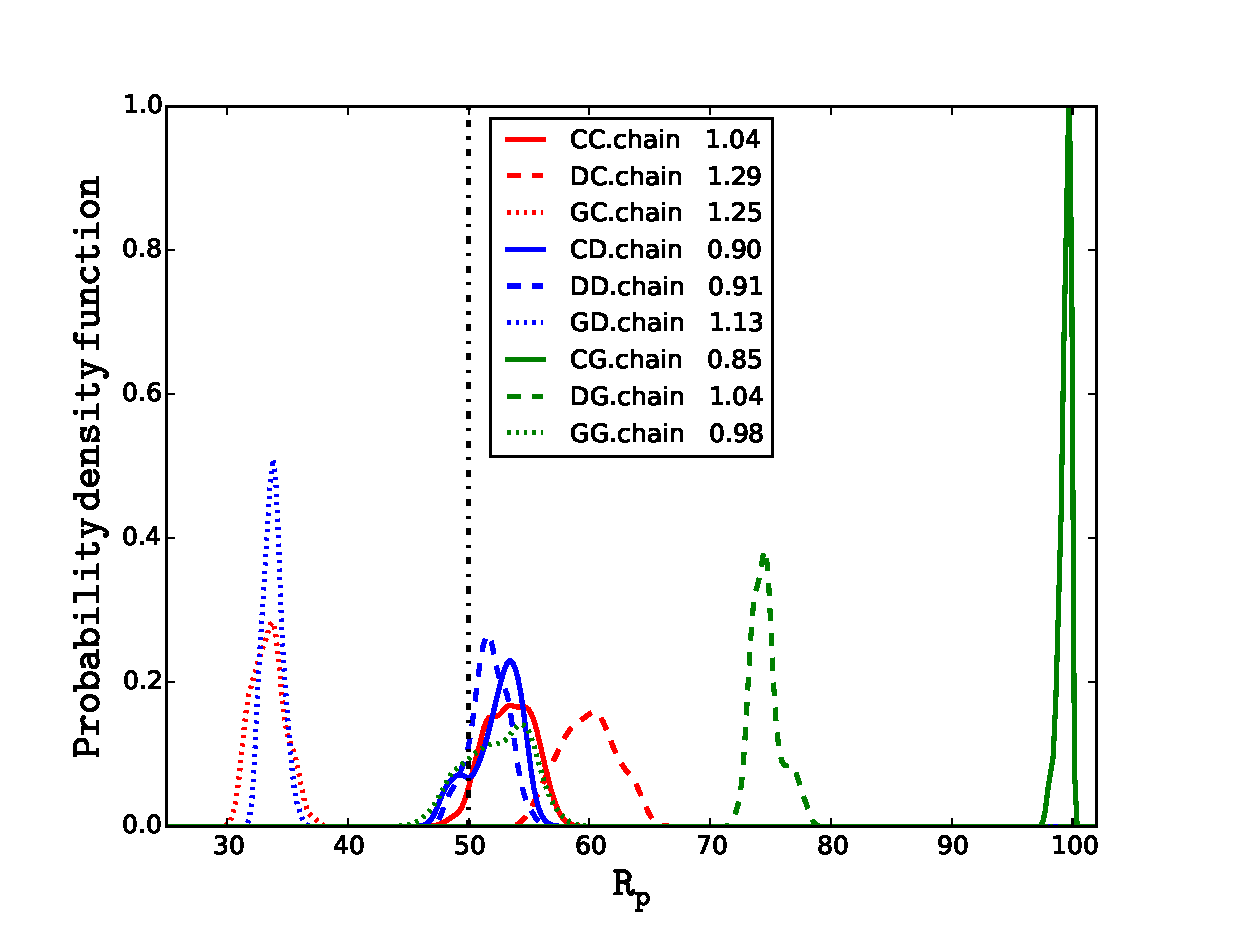
\includegraphics[width=0.9\hsize,bb=0 0 576 432
                  ]{plots/Rp4all.eps}
\caption{\label{fig:mcmc} Posterior probability distribution for the
  source size $R_p$.  The vertical line is the correct value. Same
  color represents the same dataset whereas same line style
  corresponds to same model fit.  The legend gives the reduced
  $\chi^2$ of the best fit in each case.}
\end{figure}

Figure~\ref{fig:mcmc} shows the posterior probability distribution of
$R_p$ for all nine cases, along with the minimum reduced $\chi^2$ for
each case.  The area under each curve is unity. Note that the height
of the curves are not the likelihood, they are probability densities
in parameter space.

\begin{figure}
\centering
  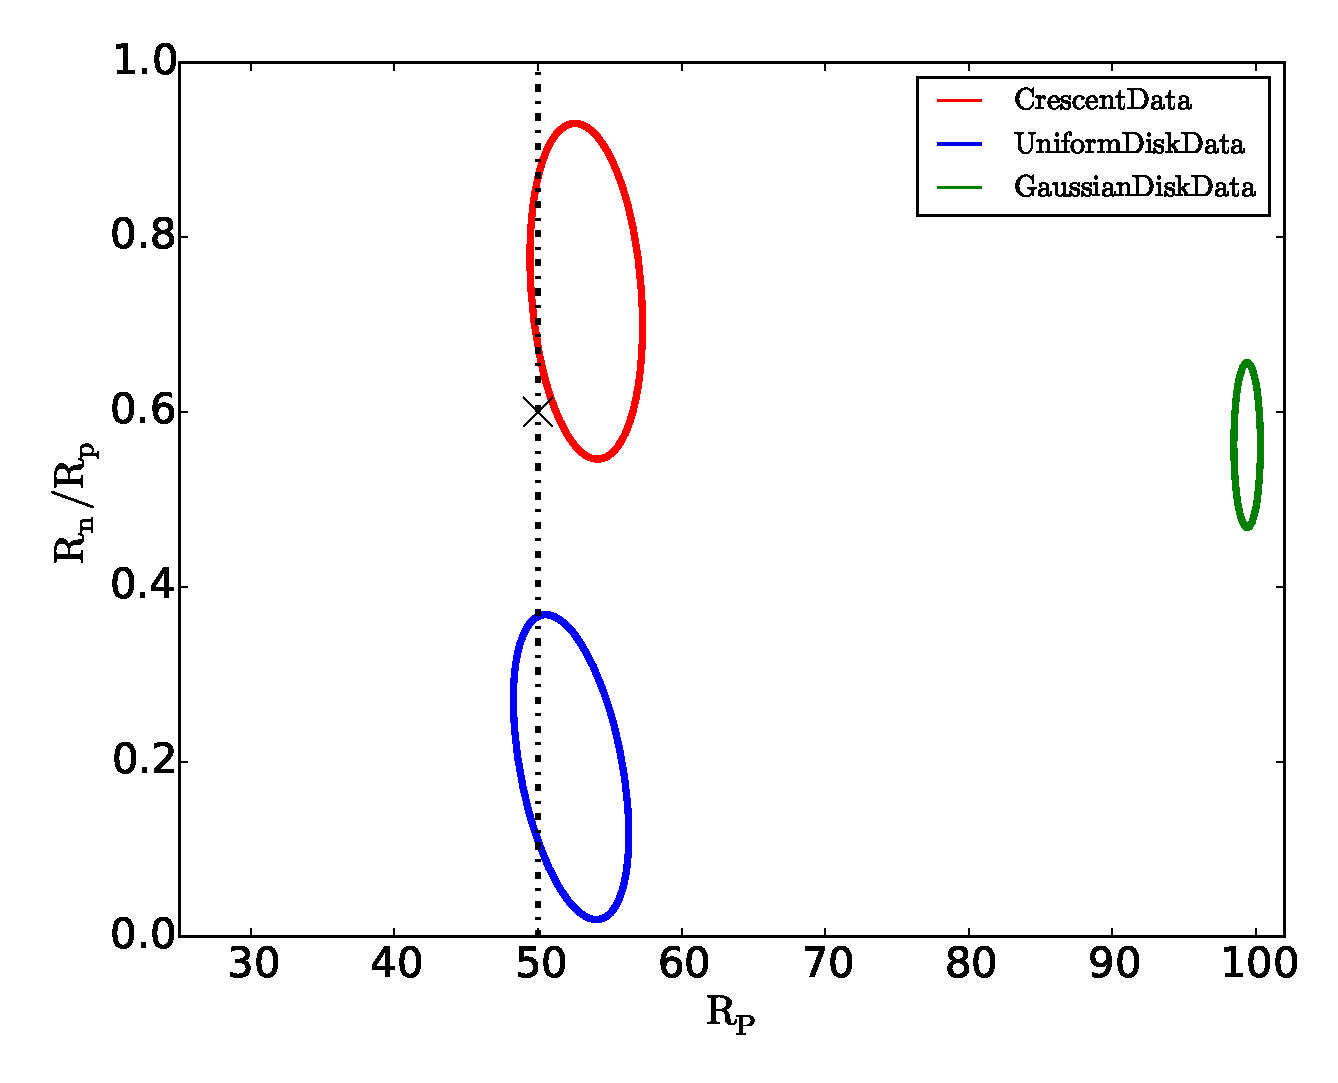
\includegraphics[width=0.9\hsize,bb=0 0 576 432
                  ]{plots/Rhalf_RnRp.eps}
  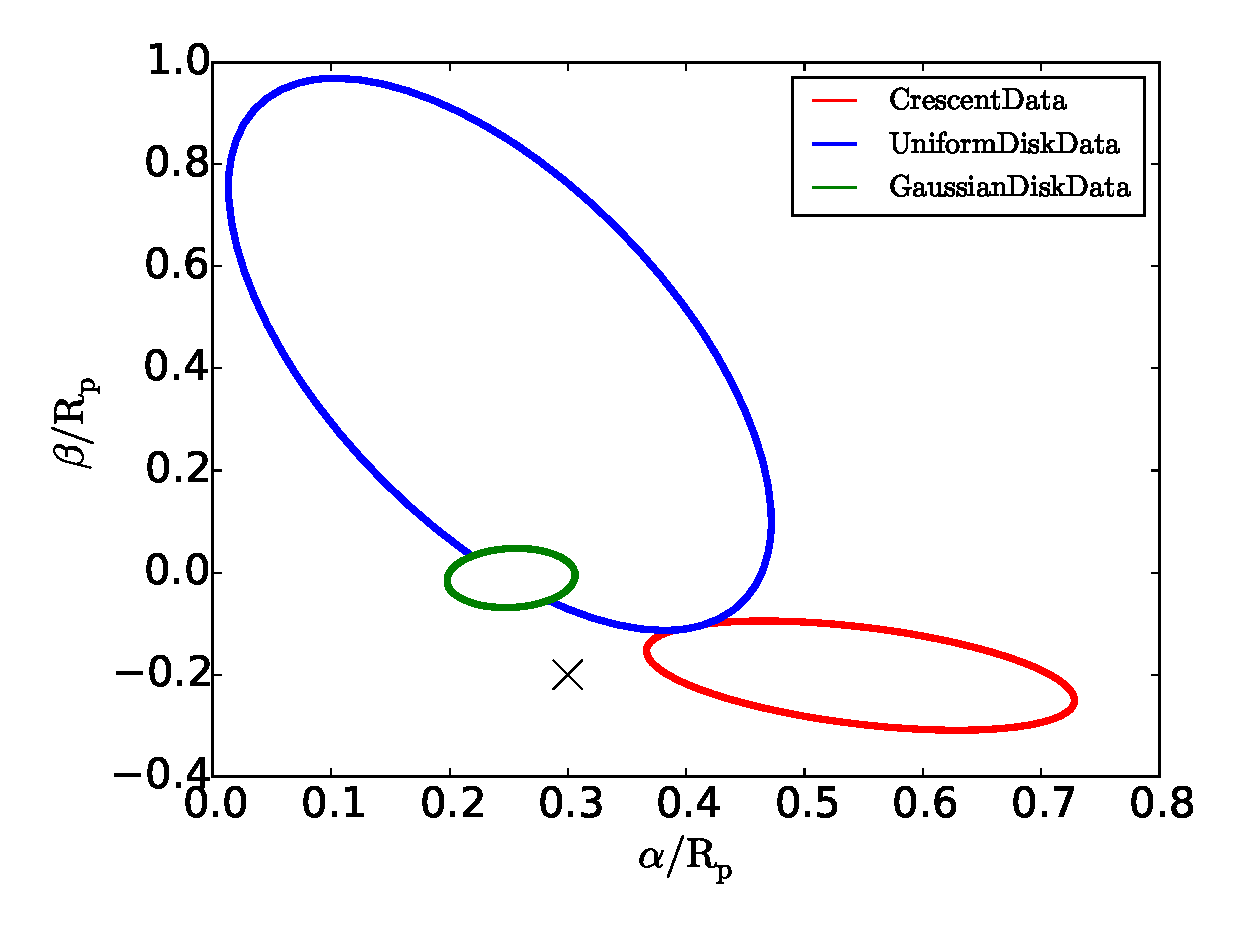
\includegraphics[width=0.9\hsize,bb=0 0 576 432
                  ]{plots/aRp_bRp.eps}
\caption{\label{fig:crescentfit} The 2$\sigma$ contours (or error ellipses)
  of the crescent model when fitting with the three different
  datasets.}
\end{figure}

Let us first consider the three cases where a crescent model was
fitted.  These are the solid curves in Figure~\ref{fig:mcmc}, with the
colours of the curves indicating the source.  Meanwhile,
Figure~\ref{fig:crescentfit} shows $2\sigma$ of the inferred parameter
values.

\begin{enumerate}

\item[1) {\bf CC}:] solid red curve in Figure~\ref{fig:mcmc} and red
  ellipses in Figure~\ref{fig:crescentfit}.  In this case, a light
  curve from a crescent source was being fitted to a crescent model.
  The fit gives reduced $\chi^2$ close to unity, as expected.  The
  recovered parameter values are near or slightly outside the
  $2\sigma$ ellipses.  This is expected, since we added a small
  systematic error, by using different caustics (though both clean
  folds) for the mock data and the model fit.  The apparent degeneracy
  between $a$ and $b$, seen in Figure~\ref{fig:crescentfit}, is also
  expected, since only the distance of the crescent's small circle
  from the caustic influences the magnification.


\item[2) {\bf CD}:] solid blue curve and blue ellipses.  Here a
  crescent model was fitted to a light curve from a uniform disc.  The
  situation is formally a crescent with $R_n=0$ and $a,b$ arbitrary,
  and this shows in the blue ellipses in the recovered parameter
  values.  The redundant parameters $\alpha$ and $\beta$, in effect, allow the
  model to partly fit the noise, and hence the $\chi^2$ is somewhat
  lower than in the previous case.

\begin{figure}
\centering
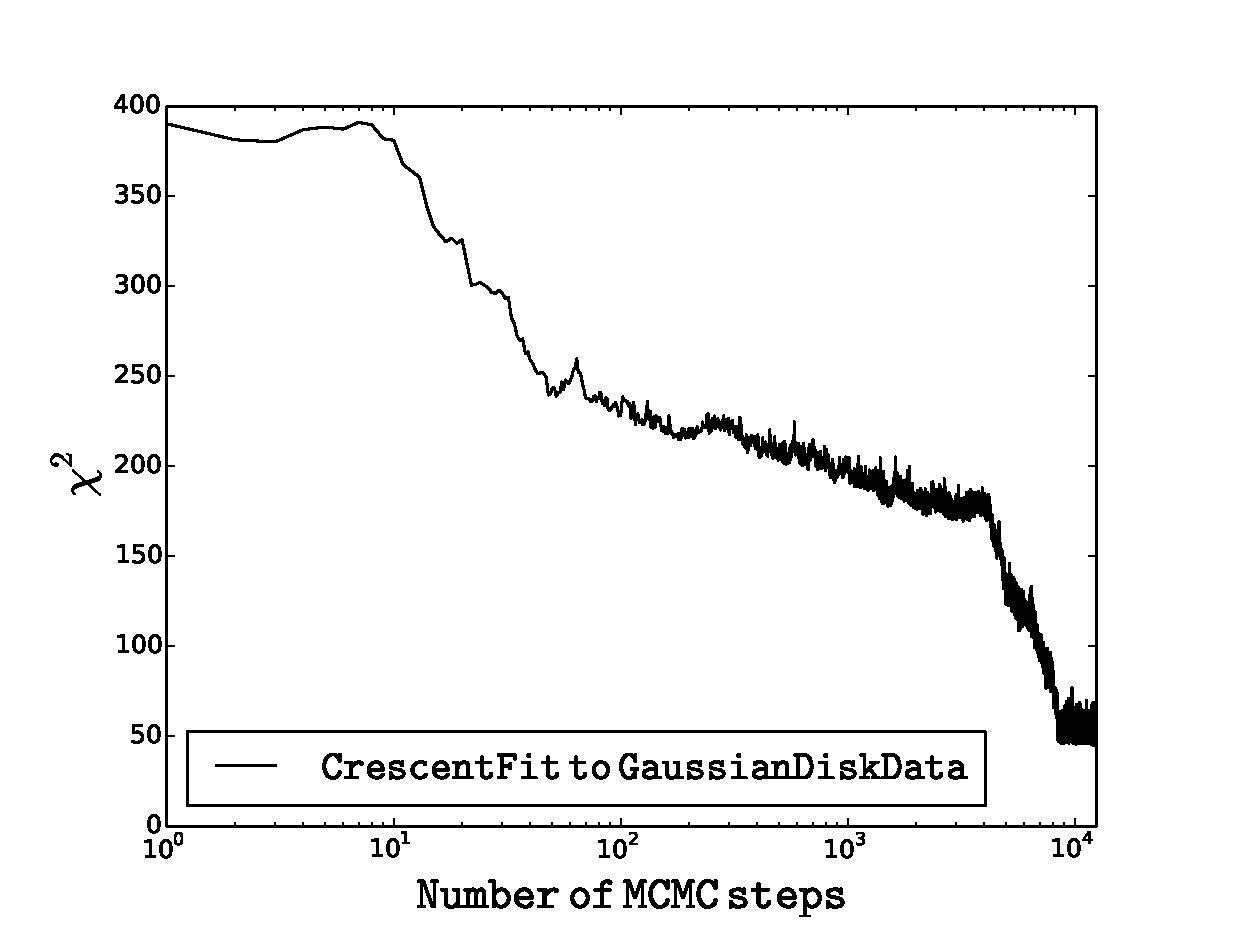
\includegraphics[width=0.9\hsize,bb=0 0 576 432
                ]{plots/burnin_cg.eps}
\caption{\label{fig:burnin} The $\chi^2$ of each step of the full MCMC
  for one case.}
\end{figure}

\item[3) {\bf CG}:] Solid green curve and green ellipses.
  Additionally, Figure~\ref{fig:burnin} shows the progress of
  reduction of $\chi^2$ in this case, where a crescent-source model is
  used to fit data from a Gaussian source.  The parameter values are
  seemingly tightly constrained, but the recovered $R_p$ is completely
  wrong, since the correct value is far from the green curve and green
  ellipses.  The reduced $\chi^2$ is only 0.85, indicative of
  over-fitting.  We can see what has happened from the red curve in
  the bottom panel of Figure~\ref{fig:mockdata}.  The best-fit model
  covers only a small part of the light curve.  That is, the fitting
  procedure has exploited the nuisance parameters to find a good fit
  to mainly noise.

\end{enumerate}

Next we consider the three cases where a disc model is fitted.  These
correspond to the dashed curves in Figure~\ref{fig:mcmc}.  There is
only one interesting parameter to fit, the disc radius $R_p$, and no
equivalent of Figure~\ref{fig:crescentfit} is needed. 

\begin{enumerate}

\item[4) {\bf DC}:] red dashed curve.  On fitting a disc model to a
  crescent-source source, the recovered $R_p$ is incorrect, but the
  reduced $\chi^2$ of 1.29 signals that the data reject the model.

\item[5) {\bf DD}:] red dashed curve.  When the correct model is
  fitted to a disc-source, the best fit $\chi^2=0.91$ is good and
  $R_p$ is recovered within the uncertainty estimate.

\item[6) {\bf DG}:] green dashed curve.  On fitting a disc model to a
  Gaussian-source model, the recovered $R_p$ is incorrect, but the
  reduced $\chi^2$ gives no signal that something is amiss.  It
  appears that a Gaussian source could mimic a uniform disc.

\end{enumerate}

Finally, we consider the three cases where a Gaussian model is fitted.
These correspond to the dotted curves in Figure~\ref{fig:mcmc}.  Again,
there is only one interesting parameter to fit, the Gaussian
$3\sigma$-radius, which we have called $R_p$.

\begin{enumerate}

\item[7) {\bf GC}:] red dotted curve.  When a Gaussian-source model is
  fitted to data from a crescent source, the recovered $R_p$ is wrong
  but the reduced $\chi^2=1.29$ shows the data rejecting the model.

\item[8) {\bf GD}:] blue dotted curve.  When a Gaussian-source model
  is fitted to data from a uniform disc, the recovered $R_p$ is wrong
  but the model is rejected anyway.

\item[9) {\bf GG}:] green dotted curve.  When data from a Gaussian is
  fitted to the correct model, $R_p$ is recovered within its estimated
  uncertainty, and the best fit reduced $\chi^2$ is close to unity.

\end{enumerate}

The above results suggest the following strategy for fitting a
lightcurve from an unknown source profile: first try a Gaussian-source
model; if the data reject that model, try a uniform disc; if the
uniform disc is also rejected by the data, try a crescent model.  Our
numerical experiments indicate --- assuming one of the three source
models is correct --- that the reduced $\chi^2$ would unmask the
correct model, \textbf{and its parameters would be correctly recovered}.



\section{Discussion}
[Mihai's contribution]\\
In the current paper we simulate and study the resulting microlensing lightcurves of geometric crescent-shaped sources 
and compare them with the microlensing lightcurves of other simple mathematically describable source profiles. 
In order to mimic the behaviour of flux of light from the source in the proximity of a fold caustic we make use of the simple approximation described in equation (5). 
The equation would exhaustively describe the magnification map and offer a good universal aproximation for the 
particular microlensing regime that we consider. 
Namely, the shape of the caustic boundary in the proximity of the source in the respective plane can be approximated with
 a line due to reason that the local radius of curvature of caustic is orders of magnitude greater than the half-light
 radius of the studied source. 
In particular cases in which the previously mentioned approximation loses its validity the impact on the quality of the 
lightcurves is not evenly distributed. The shape of the lightcurve will be maintained. 
The datapoints corresponding to the source position before and during the overlapping of the caustic will be affected by
 smaller errors than the datapoints corresponding to later times. \\

The first two source profiles that we consider are the uniform disk and symmetric gaussian source. 
Both of them can be described by a half-light radius $r_{1/2}$ and a total unlensed light flux $S_0$. 
With the two parameters constrained the one dimensional profiles as well as the lightcurves of the two source are completely determined, since no free parameter remains. 

The previous statement does not hold for a crescent source.
In the case of the crescent source there are in total five parameters: the integrated flux of the source $S_0$,
 the radii of the bright/dark disk $R_p$/$R_n$ and the displacement of the centers of the two disks on the axes perpendicular and parallel to the caustic $a$ and $b$. 

Two of the parameters can be reduced by expressing the results in terms of $S_0$ and $r_{1/2}$. 
The later being determinable for any set of parameters $R_p, R_n$ and $a^2+b^2$. Moreover, one of the displacemement 
parameters $b$ has no impact on the one dimensional profile of the source that results from the projection of the source image on an axis perpendicular to the caustic. 

Since the one dimensional source profile that corresponds to an axis perpendicular to the caustic contains exhaustively all the information regarding the source that can be revealed by the lightcurve, 
the value of the parameter $b$ does not effect the shape of the lighcurve. 

Nevertheless the $b$ parameter is relevant to the calculation of $r_{1/2}$. 
It's qualitative effect is to decrease the value of the half-light radius when the absolute value of the parameter is increased.  
With two parameters constrained and another irrelevant to the shape of the lightcurve, two free parameters remain $R_n$ and $a$. 
Figure 4 reveals that the lighcurve of a crescent source has more visible features than the other two light-curves 
corresponding to the disc and guasssian shape. The parameters $R_n$ and $a$ have strong influences on the shape of 
the microlensed lightcurve, as can be seen in figures 5, 6 and 7. Moreover, the one dimensional source profile corresponding to the direction perpendicular to the caustic reveal four characteristic points. The overlap of each of these points with the caustic leaves visible features on the lightcurve at the corresponding instances of time. In timely order the instances correspond to the start of the overlap between the caustic and the bright disk, the start of the overlap between the caustic and the dark disk, the end of the overlap between the caustic and dark disk and finally the end of the overlap between the caustic and the bright disk.          

With the different source profiles and their corresponding lightcurves studied we can change our point of view of the system to that of an observer. The observer would basically detect only the lightcurve of such as source. As described in section (Lightcurve of a crescent source) the timing of the onset and offset of the previously described periods can be used to estimate the values of the radii and one of the displacement parameters when assuming a geometric crescent, the halfwidths and one displacement parameters when assuming a constant brightness elliptical crescent and the halfwidth of the dark ellipse when assuming an elliptical gaussian crescent. All quantities can be estimated in terms of the relative velocity of the source in a direction perpendicular to the caustic.\\

The previously mentioned abstract parameters can be related to physical quantities specific to the central region of a quasar. Thus the luminous region would correspond to the bright accretion disc that surrounds the black hole. The later's gravity would cause a shadow in the bright region limited by the extent of the event horizon of the black hole. Therefore the radius of the bright disk would provide an estimate of the size of the accretion disk and the radius of the dark disc would provide and estimate of the Schwarzschild radius of the black hole. Moreover a value of the Schwarzschild radius 
can be used to estimate the mass of the black hole $M \approx \frac{\Delta t_{dark}  v_p c^2}{2G}$. In the previous 
expression the $\Delta t_{dark}$ denotes the period of overlap between the black hole shadow and fold caustic. 
$v_p$ denotes the component of the relative velocity of the source and fold which is perpendicular to the caustic.  
The respective velocity is an unknown, though it can be constrained on a case by case basis to an order of magnitude or even better. This would require the 
study of the dynamics of the stellar structure which contains the gravitational lens. A better estimate of the relative velocity would facillitate a better estimate of the effective non-rotating black hole mass associated to the black hole shadow.  


Furthermore, a simulated image of M87 presented in \citep{2012MNRAS.421.1517D} (figure 9) has been microlensed. On the resulting lightcurve the instances corresponding to the start and end of the black hole shadow and caustic overlap were distinguishable as can be seen in figure 10.
    
The parameters whose values cannot be determined due to the loss of information from the directions parallel to the 
caustic could be obtained in the eventuality in which the same source crosses multiple caustics that are not parallel. 
Multiple crossing of caustics can reveal details of the one dimensional flux profile corresponding to multiple distinct 
directions which would allow the reconstruction of the two dimensional profile analogous to the process through which an image of a CT scan is obtained.  

In case of a high quality lightcurve with insignificant noise and measurement errors, the parameters can be obtained 
by simply identifying the characterstic instances of time withought making use of the actual values of the magnification
 map. If the effect of the errors and the noise distorts the magnification time function enough so that the 
characteristic points are not identifiable with the characteristic periods still visible, the boundaries of the periods 
can be roughly estimated. To study if good estimates of the parameters can still be obtained when datapoints are
 strongly affected by the noise we propose ....        



              

[Irshad's contribution]\\

This work presents a toy model to put useful constraints on the interior structure of quasars, particularly the environment geometry of the event horizon. To carry out this analysis on real data, one needs two situations: First, a quasar which can be observed with a reasonably good telescope with high signal to noise ($\sim 150$) and second, a caustic crossing event of the quasar. These events are not rare, however, to get an isolated caustic crossing might be. As the size of the source is negligible as compared to big caustic structures in the sky, even the single fold caustic crossing is not that rare.

In this toy analysis, we used very ideal data, which might not be the case with real source but we contaminated it to match a reasonable signal to noise. 

The main emphasis of this work was the crescent model parameters, which we show can be well recovered by the maximum likelihood analysis, apart from highly degenerate $a$ and $b$ parameters. The reason of this degeneracy is also very intuitive, if one integrates parallel to the caustic to get the integrated 1D brightness profile, so if the motion of the source is either parallel or perpendicular to the caustic, one of the two parameters ($a$ and $b$) is indistinguishable and in case of angled motion of the source, these two are highly degenerate. This degeneracy can be broken if multiple crossing events of the same quasar is available. So for example, one can use the first crossing to estimate the likelihood of the four parameters and use them as priors in the second crossing and so on. In this way, one can accurately and precisely recover all four parameters. Using our toy analysis we conclude that it is feasible, in practice, to recover 2D shape of the source using a microlensing event and distinguish between symmetric and asymmetric sources.



[Contributions from authors]\\
Prasenjit Saha provided the original idea and plan for the research project as well as multiple contributions to the analysis. Mihai Tomozeiu simulated and studied the ideal behaviour of the microlensing lightcurves for the different source profiles discussed. Joachim Wambsganss provided the numerical code used by Manuel Rabold to create the magnification map and corresponding lighcurves used in the MCMC analysis, analisis that was performed by Irshad Mohammed in the last part of the presented work. 




\bibliographystyle{mn2e}

\def\apj{ApJ}
\def\apjl{ApJL}
\def\aj{AJ}
\def\mnras{MNRAS}
\def\aap{A\&A}
\def\nat{nature}
\def\araa{ARAA}
\def\pasa{PASA}
\bibliography{heap}

\end{document}
